
%!TEX root = CooperBarba2014.tex

\subsection{Discretization}

 \begin{figure}[b]
   \centering
   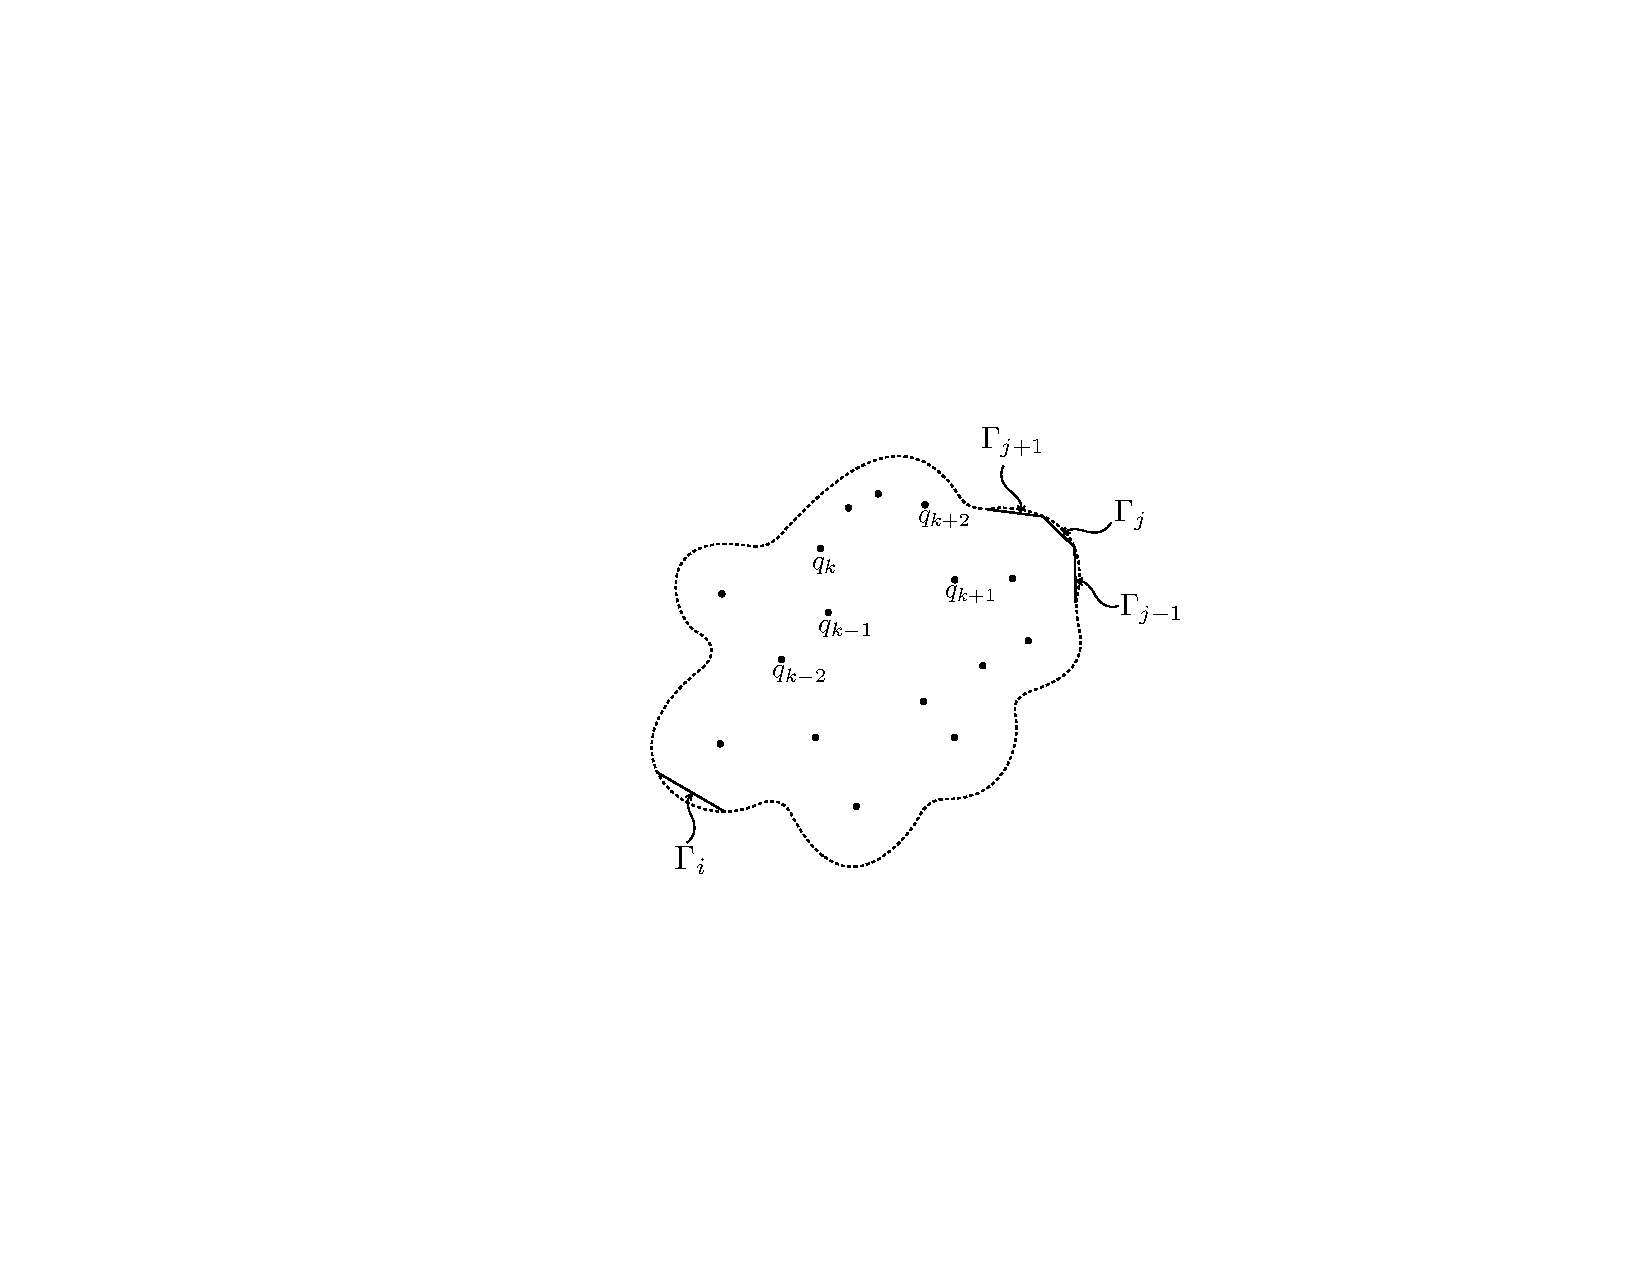
\includegraphics[width=0.4\textwidth]{Figure3.pdf} 
   \caption{Discretization of a molecular surface. $\Gamma_i$ is the panel where the collocation point resides and $\Gamma_j$ the panel being integrated.}
   \label{fig:molecule_disc}
\end{figure}

To numerically solve the system in \eqref{eq:integral_eq}, we discretize the boundaries into flat triangular panels and assume that $\phi$ and $\frac{\partial \phi}{\partial \mathbf{n}}$ are constant within those panels. The discretized form of the integral operators is as follows:
%
\begin{align} \label{eq:layers_disc}
&K_{L,\text{disc}}^{\mathbf{r}_i}(\phi(\mathbf{r}_{\Gamma})) =  \sum_{j=1}^{N_p}\phi(\mathbf{r}_{\Gamma_j})\int_{\Gamma_j} \frac{\partial}{\partial \mathbf{n}} \left[ G_L(\mathbf{r}_{i},\mathbf{r}_{\Gamma_j}) \right]\mathrm{d} \Gamma_j,  \nonumber \\
&V_{L,\text{disc}}^{\mathbf{r}_i} \left( \frac{\partial}{\partial \mathbf{n}} \phi(\mathbf{r}_{\Gamma}) \right) = \sum_{j=1}^{N_p} \frac{\partial}{\partial \mathbf{n}} \phi(\mathbf{r}_{\Gamma_j}) \int_{\Gamma_j} G_L(\mathbf{r}_{i},\mathbf{r}_{\Gamma_j})  \mathrm{d} \Gamma_j,
\end{align}

\noindent where $N_p$ is the number of discretization elements on $\Gamma$, and $\phi(\mathbf{r}_{\Gamma_j})$ and $\frac{\partial}{\partial \mathbf{n}} \phi(\mathbf{r}_{\Gamma_j})$ are the constant values of $\phi$ and $\frac{\partial \phi}{\partial \mathbf{n}}$ on panel $\Gamma_j$ (we are somewhat abusing the nomenclature here by reusing the symbol $\Gamma$, which previously referred to the complete surface). By collocating $\mathbf{r}_i$ on the center of each panel, we get a linear system of equations which looks just like those in Equations \eqref{eq:matrix_phi} and  \eqref{eq:matrix_dphi}, but its elements are sub-matrices of size $N_p \times N_p$ rather than integral operators. Looking at Figure \ref{fig:molecule_disc}, each element of a sub-matrix is an integral over one panel $\Gamma_j$, with $\mathbf{r}_i$ located at the center of the collocation panel $\Gamma_i$, as follows:

\begin{align} \label{eq:layers_element}
K_{L,ij} &= \int_{\Gamma_j} \frac{\partial}{\partial \mathbf{n}} \left[ G_L(\mathbf{r}_{\Gamma_i},\mathbf{r}_{\Gamma_j}) \right]\mathrm{d} \Gamma_j, \nonumber \\
V_{L,ij} &= \int_{\Gamma_j} G_L(\mathbf{r}_{\Gamma_i},\mathbf{r}_{\Gamma_j})  \mathrm{d} \Gamma_j.
\end{align}

The terms on the right-hand side and the unknown vectors in the discretized form of Equation \eqref{eq:matrix_phi} are sub-vectors of size $N_p$. In this case, each element is the evaluation on the collocation panel $\Gamma_i$, written as
%
\begin{align} \label{eq:vector_disc}
\phi_{1,\Gamma_1} &= \phi_1(\mathbf{r}_i), \nonumber \\
\frac{\partial}{\partial \mathbf{n}}\phi_{1,\Gamma_1} &= \frac{\partial}{\partial \mathbf{n}}\phi_1(\mathbf{r}_i), \nonumber \\
\sum_{k=0}^{N_q} \frac{q}{4\pi|\mathbf{r}_{\Gamma_1} - \mathbf{r}_k|} &= \sum_{k=0}^{N_q} \frac{q}{4\pi|\mathbf{r}_i - \mathbf{r}_k|},
\end{align}

\noindent where $\mathbf{r}_i$ is located at the center of panel $\Gamma_i$.

In our numerical solution, integrals are calculated in three ways, depending on how close the panel is to the collocation point. When the collocation point is inside the element being integrated, we use a semi-analytical technique \cite{ZhuHuangSongWhite2001}, with Gauss points placed along the edges of the element. If the integrated element is closer than $2L$ from the collocation point ---where $L = \sqrt{2\cdot \text{Area}}$--- we use a fine Gauss quadrature rule, with 19 or more points per element. Beyond a distance of $2L$, elements have only 1, 3, 4 or 7 Gauss points, depending on the case.

\subsection{Treecode-accelerated boundary element method}

Most modern implementations of the boundary element method (\bem) use Krylov methods to solve the linear system, usually a general minimal residual method (\gmres), which is agnostic to the structure of the matrix. In practice, Krylov solvers for \bem require $O(n \cdot N_p^2)$ operations to obtain the unknown vector, where $n$ is the number of iterations to get a desired residual, and is much smaller than $N_p$. The $O(N^2)$ scaling is given by a matrix-vector product (with a dense matrix) done in every iteration; this is the most time-consuming part of the algorithm, and makes \bem prohibitive for more than a few thousand discretization elements. 

But when we inspect the approximation of the integrals in  \eqref{eq:layers_element} with Gauss quadrature rules, we see that the matrix-vector product has the form of an $N$-body problem, similar to gravitational potential calculations in planetary systems. In this case, the Gauss quadrature points act analogously to planets (sources of mass) and the collocation points are analogous to the locations where the gravitational potential is computed (targets points). There are several ways to accelerate this kind of computations, for example fast-multipole methods \cite{GreengardRokhlin1987}, treecodes \cite{BarnesHut1986}, and fast-Fourier-transform methods \cite{PhillipsWhite1997}.
In our numerical solution (developed as the open-source code \pygbe), we accelerate the $N$-body calculation with a treecode \cite{BarnesHut1986,LiJohnstonKrasny2009}, making this part of the algorithm scale as $O(N\log N)$ rather than $O(N^2)$. 

The treecode algorithm groups the sources and targets in a tree-structured set of boxes and approximates interactions between far-away boxes using a series expansion---a Taylor series, in our case. This allows for controllable accuracy that depends on the number of terms used in the expansion and the multipole-acceptance criterion that defines the threshold where the distance between source and target is far enough to approximate the interactions with expansions. Details of our implementation of the treecode in \pygbe can be found in our previous work \cite{CooperBarba-share154331}.
